\section{Optimization}

\subsection{LLP}
\begin{frame}
    \frametitle{LLP}
	\begin{itemize}
		\item Many operations are mapped 1-to-1 to PLP which can translate earlier.
		\item Insert down-sample stage. 
	\end{itemize} 
\end{frame}

\begin{frame}
    \frametitle{LLP}
    \begin{figure}
		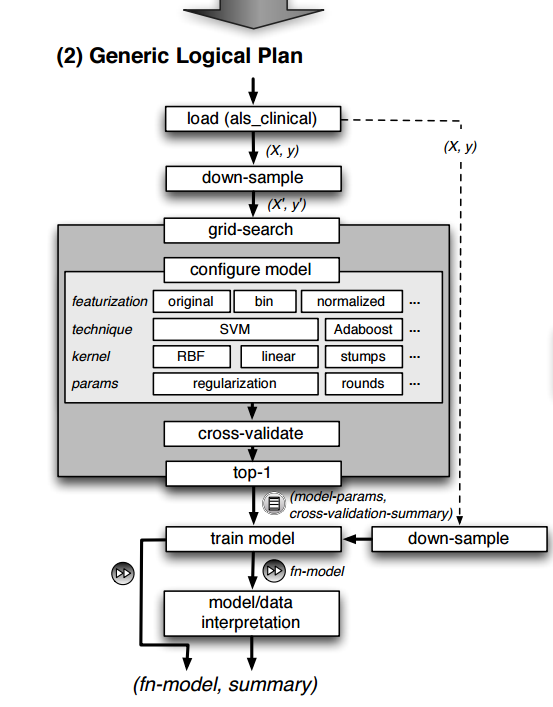
\includegraphics[scale=0.25]{figure/llp.png}
	\end{figure}
\end{frame}

\subsection{PLP}
\begin{frame}
    \frametitle{PLP}
    \begin{itemize}
		\item Transform LLP to concrete parameters and learning algorithm. 
		\item Estimate execution time based on statistical models. 
			\begin{itemize}
				\item Normalized data sets for SVM and AdaBoost. 
			\end{itemize}
		\item Use 10-folds cross validation. 
	\end{itemize}
\end{frame}

\begin{frame}
    \frametitle{PLP}
    \begin{figure}
		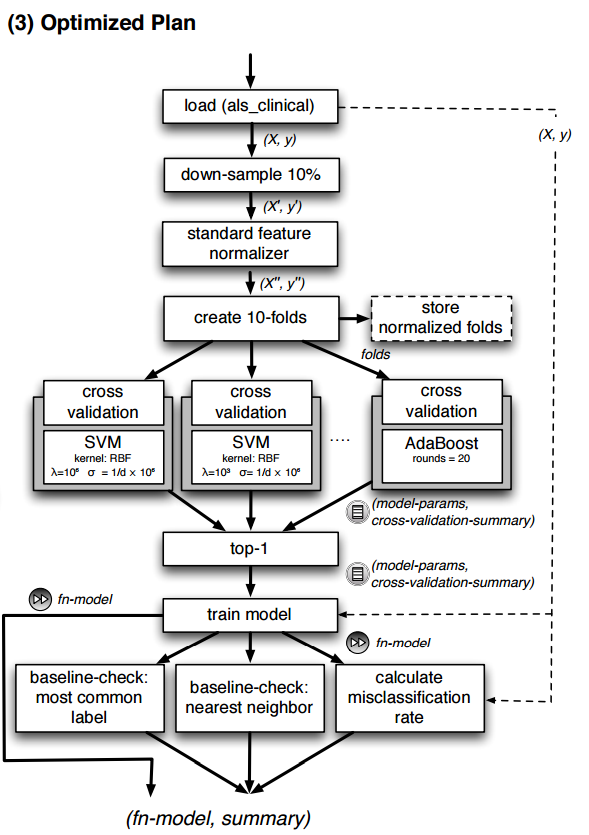
\includegraphics[scale=0.25]{figure/plp.png}
	\end{figure}
\end{frame}

\subsection{Return result}
\begin{frame}
    \frametitle{Return first result, find best in the background}
	\begin{itemize}
		\item Become more interactive. 
		\item Reduce the risk of stopping too early.  
	\end{itemize} 
\end{frame}

\subsection{Good extensibility}
\begin{frame}
    \frametitle{Good extensibility}
	\begin{itemize}
		\item A set of high-level operators to enable ML researchers to implement a wide range ML algorithms without deep systems knowledge. 
	\end{itemize} 
    \begin{figure}
		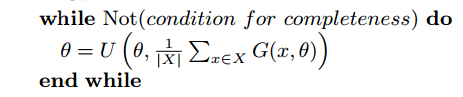
\includegraphics[scale=0.4]{figure/gdex.png}
	\end{figure}
\end{frame}
